\subsection{Knjigovodstvo}

\begin{figure}[ht]
\centering
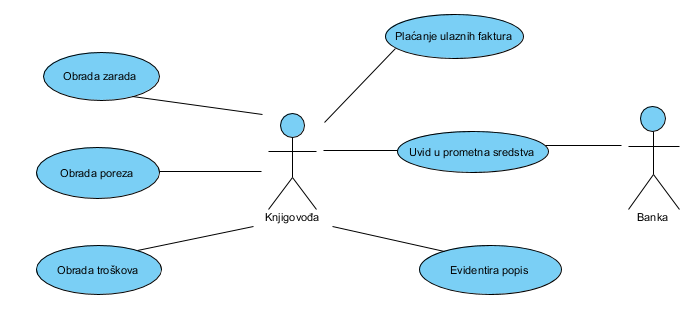
\includegraphics[width=160mm]{slike/useCaseKnjigovodstvo.png}
\caption{Dijagram slučajeva upotrebe vezanih za knjigovodstvo}
\end{figure}

\clearpage

\subsubsection{Plaćanje ulaznih faktura}

\textbf{Opis:}

Potrebno je redovno plaćati usluge dobavljača.
\newline
\textbf{Akteri:}

Knjigovođa - evidentira i vodi brigu o plaćanju ulaznih faktura
\newline
\textbf{Preduslov:}

Postoji ulazna faktura koja nije izmirena.
\newline
\textbf{Postuslov:}

Ulazna faktura je izmirena.
\newline
\textbf{Glavni tok:}

1. Knjigovođa ulazi u deo programa za knjigovodstvo, podsekcija fakture.

2. Prikazuju mu se u jednoj koloni fakture koje mi nismo izmirili, u drugoj fakture koje nama duguju.

3. Bira fakture koje trenutno mogu da se isplate, i evidentira ih kao uplaćene.

4. Uplaćuje novac na račun firmi.
\newline
\textbf{Alternativni tok:}

3. Može uplatiti iznos firmi bez navođenja konkretnih fakture, dobavljač nam skida dugove počevši od najstarije fakture.
\newline
\textbf{Napomena:}

Treba ispoštovati rokove plaćanja ako postoje. Ali generalno ne treba zapostavljati fakture.

\subsubsection{Uvid u prometna sredstva}

\textbf{Opis:}

Vodi se briga i evidencija o plaćanju naših faktura.
\newline
\textbf{Akteri:}

Banka - dnevno nam po ugovoru šalje izvod prometa sredstava

Knjigovođa - evidentira pridošle uplate za naše izlazne fakture
\newline
\textbf{Preduslov:}

Postoji izlazna faktura koja nije izmirena.
Pristigao je dnevni izvod prometa sredstava iz banke.
\newline
\textbf{Postuslov:}

Izlazna faktura je izmirena.
\newline
\textbf{Glavni tok:}

1. Knjigovođa ulazi u deo programa za knjigovodstvo, podsekcija fakture.

2. Prikazuju mu se u jednoj koloni fakture koje mi nismo izmirili, u drugoj fakture koje nama duguju.

3. Na osnovu izvoda iz banke, evidentira fakture koje su izmirene.
\newline
\textbf{Alternativni tok:}
2.1 Ako kupac nije ispoštovao rokove plaćanja treba ga kontaktirati i podsetiti.

3. Mogu nam uplatiti iznos bez navođenja konkretnih faktura, knjigovođa kupcu skida dugove počevši od najstarije fakture.

\subsubsection{Evidencija popisa}

\textbf{Opis:}

Rezultat popisa iz magacina, moguće je da se razlikuje od stanja magacina u programu. Možda je došlo do loma preparata ili je istekao rok ili se serije preparata ne poklapaju. Takođe slučajevi su i da nismo isporučili kupcu par komada lekova i on se nije bunio, ili je nama dobavljač greškom doneo više ili manje lekova.
\newline
\textbf{Akteri:}

Knjigovođa - evidentira rezultate popisa i obrađuje viškove i manjkove
\newline
\textbf{Preduslov:}

Odrađen popis u magacinu.
\newline
\textbf{Postuslov:}

Stanje magacina u programu i realno stanje se poklapaju.
\newline
\textbf{Glavni tok:}

1. Knjigovođa pristupa izveštaju balansa stanja magacina.

2. Stanja se poklapa sa popisom , idealno stanje.
\newline
\textbf{Alternativni tok:}

2. Po stanju popisa imamo manjak ili višak lekova.

3. Knjigovođa pravi interne otpremnice tj. prijemnice koje pokrivaju manjak tj. višak.

4. Ažurira stanje stanje magacina koje je u programu na stanje po popisu.
\newline
\textbf{Napomena:}

Interne prijemnice, otpremnice nisu upućene dobavljačima ili kupcima, već nam služe za zakonsko vođenje stanja robe.

\clearpage

\subsubsection{Obrada zarada}

\textbf{Opis:}

Knjigovođa obrađuje zarade zaposlenih prema politici firme. Bilo da su plate fiksne, po koeficijentima, bonusi, učinak na radu . Tu spada i porez na dohodak i doprinos. Vodi envidenciju izostanaka sa posla.
\newline
\textbf{Akteri:}

Knjigovođa - obrađuje plate u uplaćuje ih zaposlenima
\newline
\textbf{Preduslov:}

Osoblje koje je zaposleno u firmi.
\newline
\textbf{Postuslov:}

Izmireno sve vezano za plate.
\newline
\textbf{Glavni tok:}

1. Knjigovođa pristupa delu programa za obradu plata.

2. Prikazuje mu se lista zaposlenih sa platama.

3. Unosi bonuse, učinak na rad.

4. Unosi u kalkulaciju dane izostanka sa posla.

5. Uplaćuje sumu na račun zaposlenog.
\newline
\textbf{Napomena:}

Program sam popunjuje polja u vrsti zaposlenog vezana za poreze.

\subsubsection{Obrada poreza}

\textbf{Opis:}

Knjigovođa obrađuje porez koji se mesečno uplaćuje državi. To je porez na razliku u PDV-u. Ako je razlika pdv-a koji nama plaćaju kupci i pdv-a koji mi plaćamo dobavljaču pozitivna, onda tu razliku plaćamo državi. Ako je razlika negativna, onda smo u pretplati kod države.
\newline
\textbf{Akteri:}

Knjigovođa - obrađuje porez razlike u PDV-u
\newline
\textbf{Preduslov:}

Postoje uplate i isplate firme.
\newline
\textbf{Postuslov:}

Izmirena zakonska dužnost.
\newline
\textbf{Glavni tok:}

1. Knjigovođa pristupa delu programa za obradu poreza.

2. Sumu uplaćaju državi.
\newline
\textbf{Napomena:}

Deo programa za obradu poreza bi bio pogled, koji prikazuje ulazne i izlazne fakture. Sumira iznose.

\subsubsection{Obrada troškova i prihoda}

\textbf{Opis:}

Knjigovođa obrađuje rashode. To su potrošni materijali, gorivo za prevoz , reprezentativni ručkovi, materijali za poslovanje ,...
Pod prihodom se misli na ono što nam poslovanjem ostaje nakon ovih troškova i ostalih poreza. Jer godišnje se plaća 15posto državi na ostvareni prihod.
\newline
\textbf{Akteri:}

Knjigovođa - obrađuje troškove i prihode
\newline
\textbf{Preduslov:}

Postoje prihodi i rashodi firme.
\newline
\textbf{Postuslov:}

Izmirena zakonska dužnost.
\newline
\textbf{Glavni tok:}

1. Knjigovođa pristupa delu programa za obradu troškova i prihoda.

2. Vrši plaćanje svih firminih troškova.

3. Vrši plaćanje državi porez na prihod.
\newline
\textbf{Napomena:}

Deo programa za obradu troškova i prihoda bi bio pogled, koji prikazuje račune rashoda. Dok za prihode prikazuje nakon svih poreza i rashoda koliko smo prihodovali.
Porez na prihod je na godišnjem nivou, plaćanje troškova na mesečnom.

\clearpage